\chapter{{{Pengujian implementasi dan Integrasi Protokol TLS}}} 
\label{appendix:unit.test.tls}

Bagian ini menjelaskan terkait metode pengujian yang dilakukan serta hasil pengujian yang diperoleh.

\section{Kasus Uji T2.1}

Algoritma pengujian \ref{alg:unit.test.t2.1} menjelaskan proses pengujian TLS \emph{handshake} antara Alice dan Bob. Pengujian ini dilakukan untuk memastikan bahwa kunci yang dihasilkan oleh Alice dan Bob sama.

\begin{algorithm}
  \caption{Algoritme Pengujian Kasus Uji T2.1}
  \label{alg:unit.test.t2.1}
  \begin{algorithmic}
    \State $cert, prk \gets generatePairCertificate()$
    \State $socket \gets \text{UnixSocket}()$ 
    \State $tls_{alice} \gets \text{TLSApplication}(socket, \text{'client'}, cert)$ 
    \State $tls_{bob} \gets \text{TLSApplication}(socket, \text{'server'}, cert, prk)$
    \State
    \State $tls_{bob}.\text{listen}()$ \Comment {Bob melakukan listen pada socket} 
    \State $tls_{alice}.\text{connect}()$ \Comment {Alice dan Bob melakukan proses handshake} 
    \State
    \State \textbf{assert} $tls_{alice}.\text{handshakeSuccess} \land tls_{bob}.\text{handshakeSuccess}$
    \State \textbf{assert} $tls_{alice}.\text{keyReadChaos} = tls_{bob}.\text{keyWriteChaos}$
    \State \textbf{assert} $tls_{alice}.\text{keyWriteChaos} = tls_{bob}.\text{keyReadChaos}$
    \State \textbf{assert} $tls_{alice}.\text{ctrReadChaos} = tls_{bob}.\text{ctrWriteChaos}$
    \State \textbf{assert} $tls_{alice}.\text{ctrWriteChaos} = tls_{bob}.\text{ctrReadChaos}$
    \State \textbf{assert} $tls_{alice}.\text{keyMac} = tls_{bob}.\text{keyMac}$
  \end{algorithmic}
\end{algorithm}

Hasil dari pengujian ini ditunjukan oleh gambar \ref{fig:unit.test.t2.1}. Pada gambar tersebut, terlihat bahwa pengujian berhasil.

\begin{figure}[ht]
  \centering
  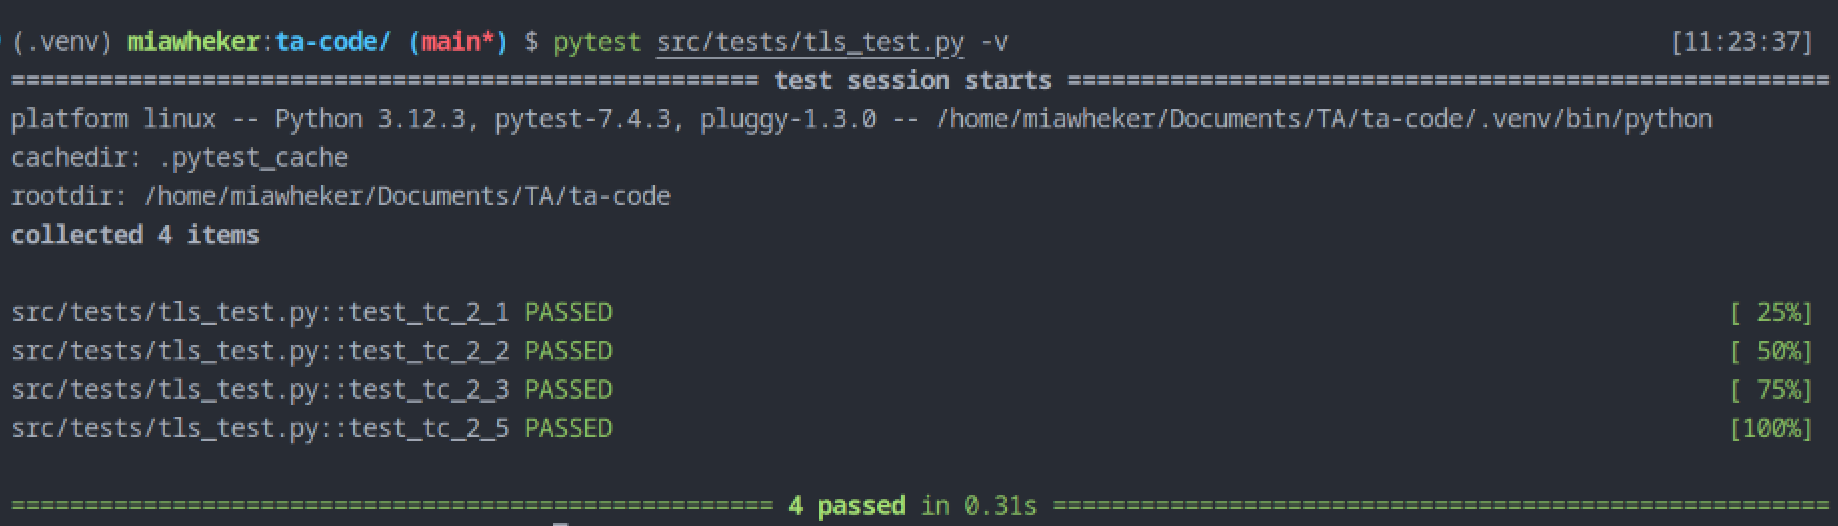
\includegraphics[width=\textwidth]{chapters/res/appendix-4/tls_test.png}
  \caption{Hasil Pengujian Kasus Uji T2.1, T2.2, T2.3, dan T2.5}
  \label{fig:unit.test.t2.1}
\end{figure}

\section{Kasus Uji T2.2}

Algoritma pengujian \ref{alg:unit.test.t2.2} menjelaskan proses pengujian TLS antara Alice dan Bob. Pengujian ini dilakukan untuk memastikan bahwa pesan teks yang dikirim oleh Alice diterima oleh Bob dan sebaliknya. Hasil dari pengujian ini ditunjukan oleh gambar \ref{fig:unit.test.t2.1}. Pada gambar tersebut, terlihat bahwa pengujian berhasil.

\begin{algorithm}
  \caption{Algoritme Pengujian Kasus Uji T2.2}
  \label{alg:unit.test.t2.2}
  \begin{algorithmic}
    \State $cert, prk \gets generatePairCertificate()$
    \State $socket \gets \text{UnixSocket}()$ 
    \State $tls_{alice} \gets \text{TLSApplication}(socket, \text{'client'}, cert)$ 
    \State $tls_{bob} \gets \text{TLSApplication}(socket, \text{'server'}, cert, prk)$
    \State
    \State $tls_{bob}.\text{listen}()$ \Comment {Bob melakukan listen pada socket} 
    \State $tls_{alice}.\text{connect}()$ \Comment {Alice dan Bob melakukan proses handshake} 
    \State
    \State $tls_{alice}.\text{send}(\text{'Hello, Server!'})$
    \State $txt_{bob} \gets tls_{bob}.\text{recv}(14)$
    \State
    \State $tls_{bob}.\text{send}(\text{'Hello, Client!'})$
    \State $txt_{alice} \gets tls_{alice}.\text{recv}(14)$
    \State
    \State \textbf{assert} $txt_{alice} = \text{'Hello, Client!'}$
    \State \textbf{assert} $txt_{bob} = \text{'Hello, Server!'}$
  \end{algorithmic}
\end{algorithm}

\section{Kasus Uji T2.3}

Algoritma pengujian \ref{alg:unit.test.t2.3} menjelaskan proses pengujian TLS antara Alice dan Bob. Pengujian ini dilakukan untuk memastikan bahwa pesan biner yang dikirim oleh Alice diterima oleh Bob dan sebaliknya. Hasil dari pengujian ini ditunjukan oleh gambar \ref{fig:unit.test.t2.1}. Pada gambar tersebut, terlihat bahwa pengujian berhasil.

\begin{algorithm}
  \caption{Algoritme Pengujian Kasus Uji T2.3}
  \label{alg:unit.test.t2.3}
  \begin{algorithmic}
    \State $cert, prk \gets generatePairCertificate()$
    \State $socket \gets \text{UnixSocket}()$ 
    \State $tls_{alice} \gets \text{TLSApplication}(socket, \text{'client'}, cert)$ 
    \State $tls_{bob} \gets \text{TLSApplication}(socket, \text{'server'}, cert, prk)$
    \State
    \State $tls_{bob}.\text{listen}()$ \Comment {Bob melakukan listen pada socket} 
    \State $tls_{alice}.\text{connect}()$ \Comment {Alice dan Bob melakukan proses handshake} 
    \State
    \State $msg_1 \gets \text{generateRandomBytes}(1024)$
    \State $tls_{alice}.\text{send}(msg_1)$
    \State $txt_{bob} \gets tls_{bob}.\text{recv}(1024)$
    \State
    \State $msg_2 \gets \text{generateRandomBytes}(1024)$
    \State $tls_{bob}.\text{send}(msg_2)$
    \State $txt_{alice} \gets tls_{alice}.\text{recv}(14)$
    \State
    \State \textbf{assert} $txt_{alice} = msg_2$
    \State \textbf{assert} $txt_{bob} = msg_1$
  \end{algorithmic}
\end{algorithm}

\section{Kasus Uji T2.4}

Algoritma pengujian \ref{alg:unit.test.t2.4} menjelaskan proses pengujian TLS \emph{handshake} antara Alice dan Bob saat adanya \emph{tampering} pada \emph{frame} \emph{ServerKeyExchange}. Pengujian ini dilakukan untuk memastikan bahwa \emph{handshake} akan gagal saat ada \emph{tampering} pada \emph{frame} \emph{ServerKeyExchange}. 

\begin{algorithm}
  \caption{Algoritme Pengujian Kasus Uji T2.4}
  \label{alg:unit.test.t2.4}
  \begin{algorithmic}
    \State $cert, prk \gets generatePairCertificate()$
    \State $socket_1 \gets \text{UnixSocket}()$
    \State $socket_2 \gets \text{UnixSocket}()$
    \State $tls_{alice} \gets \text{TLSApplication}(socket_1, \text{'client'}, cert)$ 
    \State $tls_{bob} \gets \text{TLSApplication}(socket_2, \text{'server'}, cert, prk)$
    \State $mitm \gets \text{MITMProxy}(socket_1, socket_2)$
    \State
    \State $tls_{bob}.\text{listen}()$ \Comment {Bob melakukan listen pada socket} 
    \State $tls_{alice}.\text{connect}()$ \Comment {Alice dan Bob melakukan proses handshake} 
    \State
    \State $mitm.\text{forward}(2)$ \Comment {MITM meneruskan \emph{frame} ClientHello ke socket 2}
    \State $mitm.\text{forward}(1)$ \Comment {MITM meneruskan \emph{frame} ServerHello ke socket 1}
    \State $mitm.\text{forward}(1)$ \Comment {MITM meneruskan \emph{frame} Certificate ke socket 1}
    \State
    \State $keyEx \gets mitm.\text{getFrame}()$ \Comment {MITM mengambil \emph{frame} ServerKeyExchange}
    \State $keyEx.ecdh.\text{Y} \gets -keyEx.ecdh.Y$ \Comment {Mengubah nilai parameter ECDH}
    \State $mitm.\text{send}(1, keyEx)$
    \State
    \State $mitm.\text{forward}(1)$ \Comment {MITM meneruskan \emph{frame} ServerHelloDone}
    \State $mitm.\text{forward}(2)$ \Comment {MITM meneruskan \emph{frame} ClientKeyExchange}
    \State $mitm.\text{forward}(2)$ \Comment {MITM meneruskan \emph{frame} Finished (dari client)}
    \State
    \State $alert \gets mitm.\text{getFrame}()$
    \State $mitm.\text{send}(1, alert)$
    \State
    \State \textbf{assert} $\lnot tls_{alice}.\text{handshakeSuccess} \land \lnot tls_{bob}.\text{handshakeSuccess}$
    \State \textbf{assert} $alert.\text{type} = \text{ContentType.alert}$
    \State \textbf{assert} $alert.\text{level} = \text{AlertLevel.fatal}$
    \State \textbf{assert} $alert.\text{description} = \text{AlertDescription.handshake\_failure}$
  \end{algorithmic}
\end{algorithm}

Hasil dari pengujian ini ditunjukan oleh gambar \ref{fig:unit.test.t2.4}. Pada gambar tersebut, terlihat bahwa pengujian berhasil.

\begin{figure}[ht]
  \centering
  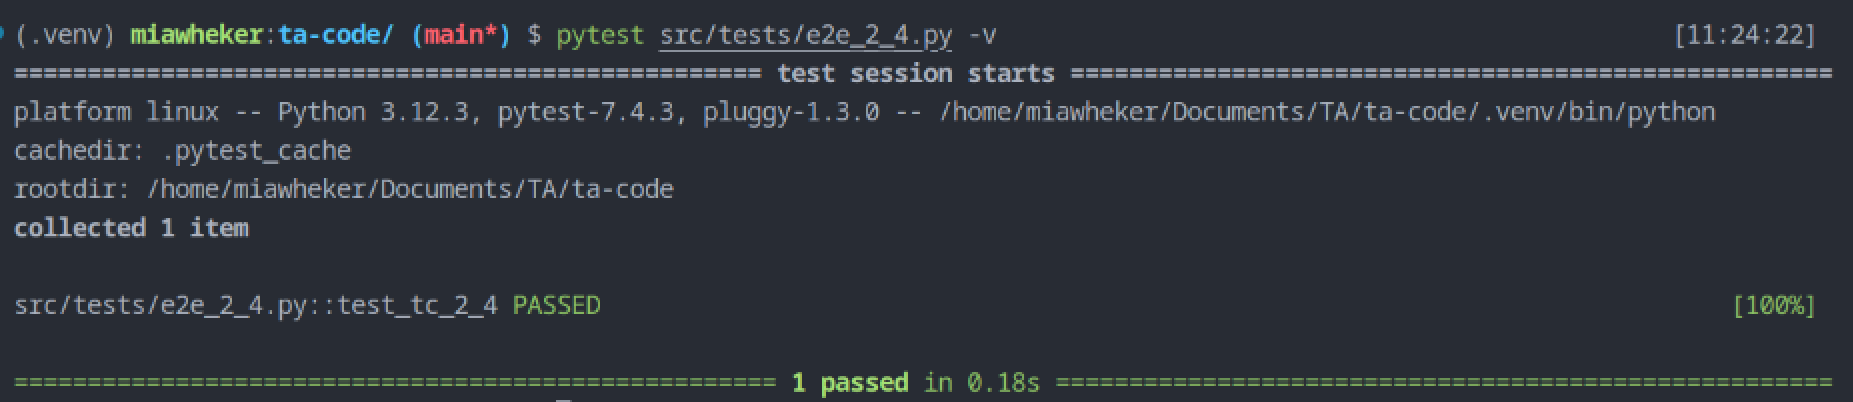
\includegraphics[width=\textwidth]{chapters/res/appendix-4/2.4.png}
  \caption{Hasil Pengujian Kasus Uji T2.4}
  \label{fig:unit.test.t2.4}
\end{figure}

\section{Kasus Uji T2.5}

Kasus uji ini menjelaskan proses pengujian TLS \emph{handshake} antara Alice dan Bob saat adanya pengubahan \emph{private key} pada \emph{frame} \emph{ServerKeyExchange}. Pengujian ini dilakukan untuk memastikan bahwa \emph{handshake} akan gagal saat ada pengubahan \emph{private key} pada \emph{frame} \emph{ServerKeyExchange}.

\begin{algorithm}
  \caption{Algoritme Pengujian Kasus Uji T2.5}
  \label{alg:unit.test.t2.5}
  \begin{algorithmic}
    \State $cert_1, prk_1 \gets generatePairCertificate()$
    \State $cert_2, prk_2 \gets generatePairCertificate()$
    \State $socket \gets \text{UnixSocket}()$
    \State $tls_{alice} \gets \text{TLSApplication}(socket, \text{'client'}, cert_1)$ 
    \State $tls_{bob} \gets \text{TLSApplication}(socket, \text{'server'}, cert_1, prk_2)$
    \State
    \State $tls_{bob}.\text{listen}()$ \Comment {Bob melakukan listen pada socket} 
    \State $tls_{alice}.\text{connect}()$ \Comment {Alice dan Bob melakukan proses handshake} 
    \State
    \State
    \State \textbf{assert} $\lnot tls_{alice}.\text{handshakeSuccess} \land \lnot tls_{bob}.\text{handshakeSuccess}$
  \end{algorithmic}
\end{algorithm}

Hasil dari pengujian ini ditunjukan oleh gambar \ref{fig:unit.test.t2.1}. Pada gambar tersebut, terlihat bahwa pengujian berhasil.

\section{Kasus Uji T2.6}

Kasus uji ini menjelaskan proses pengujian TLS saat menerima pesan dengan MAC yang tidak valid. Kasus uji ini dijelaskan melalui algoritme pengujian \ref{alg:unit.test.t2.6}. Hasil dari pengujian ini ditunjukan oleh gambar \ref{fig:unit.test.t2.4}. Pada gambar tersebut, terlihat bahwa pengujian berhasil.

\begin{algorithm}
  \caption{Algoritme Pengujian Kasus Uji T2.6}
  \label{alg:unit.test.t2.6}
  \begin{algorithmic}
    \State $cert, prk \gets generatePairCertificate()$
    \State $socket_1 \gets \text{UnixSocket}()$
    \State $socket_2 \gets \text{UnixSocket}()$
    \State $tls_{alice} \gets \text{TLSApplication}(socket_1, \text{'client'}, cert)$ 
    \State $tls_{bob} \gets \text{TLSApplication}(socket_2, \text{'server'}, cert, prk)$
    \State $mitm \gets \text{MITMProxy}(socket_1, socket_2)$
    \State
    \State $tls_{bob}.\text{listen}()$ \Comment {Bob melakukan listen pada socket} 
    \State $tls_{alice}.\text{connect}()$ \Comment {Alice dan Bob melakukan proses handshake} 
    \State
    \State $mitm.\text{forward}(2)$ \Comment {MITM meneruskan \emph{frame} ClientHello ke socket 2}
    \State $mitm.\text{forward}(1)$ \Comment {MITM meneruskan \emph{frame} ServerHello ke socket 1}
    \State $mitm.\text{forward}(1)$ \Comment {MITM meneruskan \emph{frame} Certificate ke socket 1}
    \State $mitm.\text{forward}(1)$ \Comment {MITM meneruskan \emph{frame} ServerKeyExchange ke socket 1}
    \State $mitm.\text{forward}(1)$ \Comment {MITM meneruskan \emph{frame} ServerHelloDone ke socket 1}
    \State $mitm.\text{forward}(2)$ \Comment {MITM meneruskan \emph{frame} ClientKeyExchange ke socket 2}
    \State $mitm.\text{forward}(2)$ \Comment {MITM meneruskan \emph{frame} ChangeCipherSpec ke socket 2}
    \State $mitm.\text{forward}(2)$ \Comment {MITM meneruskan \emph{frame} Finished (dari client)}
    \State $mitm.\text{forward}(1)$ \Comment {MITM meneruskan \emph{frame} ChangeCipherSpec ke socket 1}
    \State $mitm.\text{forward}(1)$ \Comment {MITM meneruskan \emph{frame} Finished (dari server)}
    \State
    \State $tls_{bob}.send(\text{'Hello, World!'})$
    \State $frame \gets mitm.\text{getFrame}()$
    \State $frame.mac[10] \gets frame.mac[10] \oplus \text{FF}_{16}$ \Comment {Ubah Nilai MAC}
    \State $mitm.\text{send}(1, frame)$
    \State
    \State $alert \gets mitm.\text{getFrame}()$
    \State \textbf{assert} $alert.\text{type} = \text{ContentType.alert}$
    \State \textbf{assert} $alert.\text{level} = \text{AlertLevel.fatal}$
    \State \textbf{assert} $alert.\text{description} = \text{AlertDescription.bad\_record\_mac}$
  \end{algorithmic}
\end{algorithm}

\begin{figure}[ht]
  \centering
  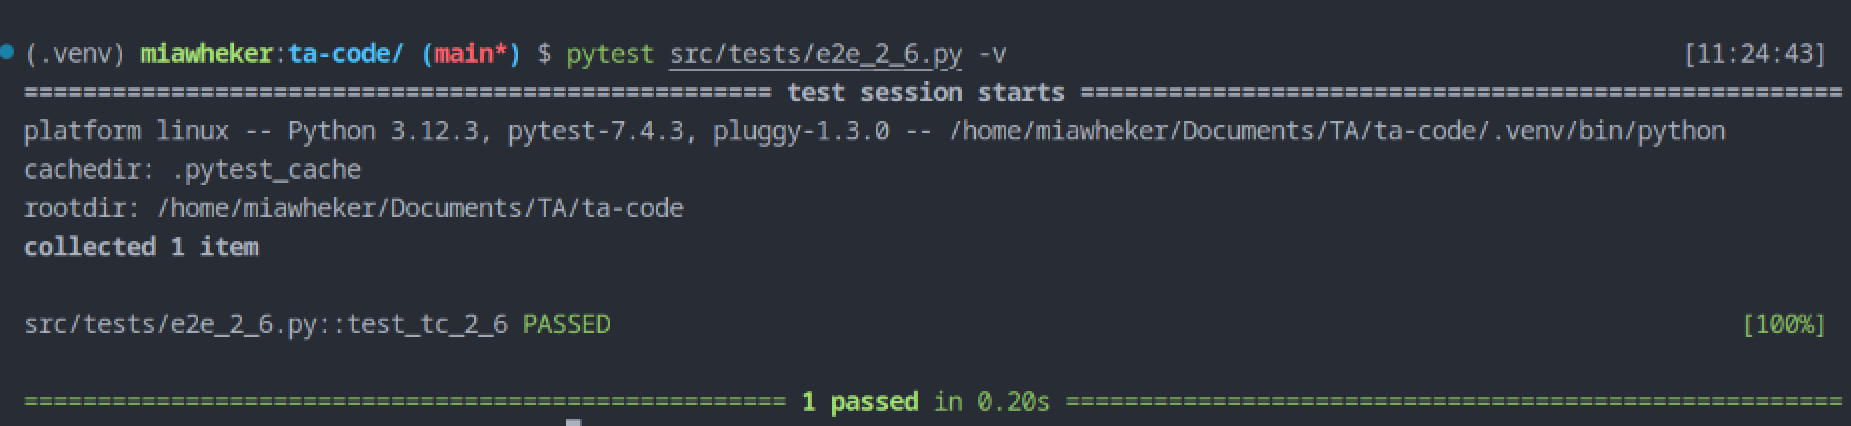
\includegraphics[width=\textwidth]{chapters/res/appendix-4/2.6.png}
  \caption{Hasil Pengujian Kasus Uji T2.4}
  \label{fig:unit.test.t2.6}
\end{figure}

\section{Kasus Uji T2.7}

Kasus uji ini memastikan pengiriman pesan masih tetap dapat berlangsung setelah menerima \emph{frame} dengan MAC tidak valid. Algoritme \ref{alg:unit.test.t2.7} menjelaskan terkait implementasi kasus uji ini. Hasil dari pengujian ini ditunjukan oleh gambar \ref{fig:unit.test.t2.4}. Pada gambar tersebut, terlihat bahwa pengujian berhasil.


\begin{algorithm}
  \caption{Algoritme Pengujian Kasus Uji T2.7}
  \label{alg:unit.test.t2.7}
  \begin{algorithmic}
    \State $cert, prk \gets generatePairCertificate()$
    \State $socket_1 \gets \text{UnixSocket}()$
    \State $socket_2 \gets \text{UnixSocket}()$
    \State $tls_{alice} \gets \text{TLSApplication}(socket_1, \text{'client'}, cert)$ 
    \State $tls_{bob} \gets \text{TLSApplication}(socket_2, \text{'server'}, cert, prk)$
    \State $mitm \gets \text{MITMProxy}(socket_1, socket_2)$
    \State
    \State $tls_{bob}.\text{listen}()$ \Comment {Bob melakukan listen pada socket} 
    \State $tls_{alice}.\text{connect}()$ \Comment {Alice dan Bob melakukan proses handshake} 
    \State
    \State $mitm.\text{forward}(2)$ \Comment {MITM meneruskan \emph{frame} ClientHello ke socket 2}
    \State $mitm.\text{forward}(1)$ \Comment {MITM meneruskan \emph{frame} ServerHello ke socket 1}
    \State $mitm.\text{forward}(1)$ \Comment {MITM meneruskan \emph{frame} Certificate ke socket 1}
    \State $mitm.\text{forward}(1)$ \Comment {MITM meneruskan \emph{frame} ServerKeyExchange ke socket 1}
    \State $mitm.\text{forward}(1)$ \Comment {MITM meneruskan \emph{frame} ServerHelloDone ke socket 1}
    \State $mitm.\text{forward}(2)$ \Comment {MITM meneruskan \emph{frame} ClientKeyExchange ke socket 2}
    \State $mitm.\text{forward}(2)$ \Comment {MITM meneruskan \emph{frame} ChangeCipherSpec ke socket 2}
    \State $mitm.\text{forward}(2)$ \Comment {MITM meneruskan \emph{frame} Finished (dari client)}
    \State $mitm.\text{forward}(1)$ \Comment {MITM meneruskan \emph{frame} ChangeCipherSpec ke socket 1}
    \State $mitm.\text{forward}(1)$ \Comment {MITM meneruskan \emph{frame} Finished (dari server)}
    \State
    \State $tls_{bob}.send(\text{'Hello, World!'})$
    \State $frame \gets mitm.\text{getFrame}()$
    \State $frameOriginal \gets frame$
    \State $frame.mac[10] \gets frame.mac[10] \oplus \text{FF}_{16}$ \Comment {Ubah Nilai MAC}
    \State $mitm.\text{send}(1, frame)$
    \State $mitm.\text{send}(1, frameOriginal)$
    \State
    \State $txt_{alice} \gets tls_{alice}.\text{recv}(13)$
    \State \textbf{assert} $txt_{alice} = \text{'Hello, World!'}$
  \end{algorithmic}
\end{algorithm}

\begin{figure}[ht]
  \centering
  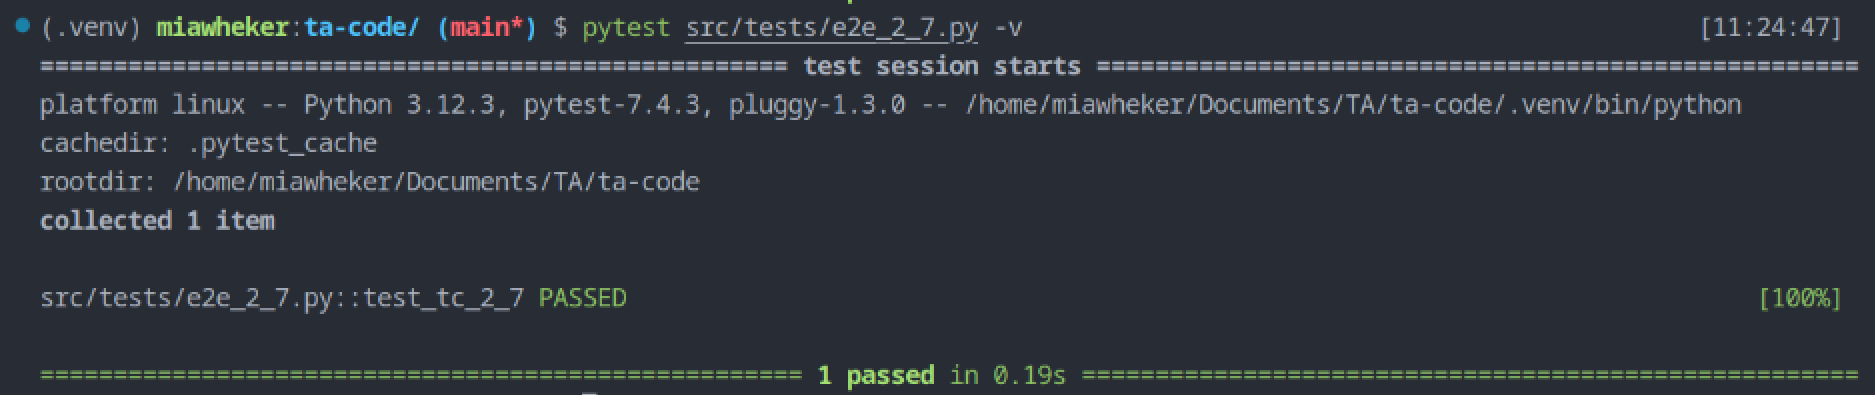
\includegraphics[width=\textwidth]{chapters/res/appendix-4/2.7.png}
  \caption{Hasil Pengujian Kasus Uji T2.7}
  \label{fig:unit.test.t2.7}
\end{figure}

\section{Kasus Uji T2.8}

Kasus uji ini menguji terkait dengan \emph{replay attack} pada protokol TLS. Algoritme \ref{alg:unit.test.t2.8} menjelaskan terkait implementasi kasus uji ini. Hasil dari pengujian ini ditunjukan oleh gambar \ref{fig:unit.test.t2.8}. Pada gambar tersebut, terlihat bahwa pengujian berhasil.


\begin{algorithm}
  \caption{Algoritme Pengujian Kasus Uji T2.8}
  \label{alg:unit.test.t2.8}
  \begin{algorithmic}
    \State $cert, prk \gets generatePairCertificate()$
    \State $socket_1 \gets \text{UnixSocket}()$
    \State $socket_2 \gets \text{UnixSocket}()$
    \State $tls_{alice} \gets \text{TLSApplication}(socket_1, \text{'client'}, cert)$ 
    \State $tls_{bob} \gets \text{TLSApplication}(socket_2, \text{'server'}, cert, prk)$
    \State $mitm \gets \text{MITMProxy}(socket_1, socket_2)$
    \State
    \State $tls_{bob}.\text{listen}()$ \Comment {Bob melakukan listen pada socket} 
    \State $tls_{alice}.\text{connect}()$ \Comment {Alice dan Bob melakukan proses handshake} 
    \State
    \State $mitm.\text{forward}(2)$ \Comment {MITM meneruskan \emph{frame} ClientHello ke socket 2}
    \State $mitm.\text{forward}(1)$ \Comment {MITM meneruskan \emph{frame} ServerHello ke socket 1}
    \State $mitm.\text{forward}(1)$ \Comment {MITM meneruskan \emph{frame} Certificate ke socket 1}
    \State $mitm.\text{forward}(1)$ \Comment {MITM meneruskan \emph{frame} ServerKeyExchange ke socket 1}
    \State $mitm.\text{forward}(1)$ \Comment {MITM meneruskan \emph{frame} ServerHelloDone ke socket 1}
    \State $mitm.\text{forward}(2)$ \Comment {MITM meneruskan \emph{frame} ClientKeyExchange ke socket 2}
    \State $mitm.\text{forward}(2)$ \Comment {MITM meneruskan \emph{frame} ChangeCipherSpec ke socket 2}
    \State $mitm.\text{forward}(2)$ \Comment {MITM meneruskan \emph{frame} Finished (dari client)}
    \State $mitm.\text{forward}(1)$ \Comment {MITM meneruskan \emph{frame} ChangeCipherSpec ke socket 1}
    \State $mitm.\text{forward}(1)$ \Comment {MITM meneruskan \emph{frame} Finished (dari server)}
    \State
    \State $tls_{bob}.send(\text{'Hello, World!'})$
    \State $frame \gets mitm.\text{getFrame}()$
    \State $mitm.\text{send}(1, frame)$
    \State
    \State $txt_{alice} \gets tls_{alice}.\text{recv}(13)$
    \State $mitm.\text{send}(1, frame)$ \Comment {Melakukan Replay Attack}
    \State
    \State $alert \gets mitm.\text{getFrame}()$
    \State \textbf{assert} $txt_{alice} = \text{'Hello, World!'}$
    \State \textbf{assert} $alert.\text{type} = \text{ContentType.alert}$
    \State \textbf{assert} $alert.\text{level} = \text{AlertLevel.fatal}$
    \State \textbf{assert} $alert.\text{description} = \text{AlertDescription.bad\_record\_mac}$    
  \end{algorithmic}
\end{algorithm}

\begin{figure}[ht]
  \centering
  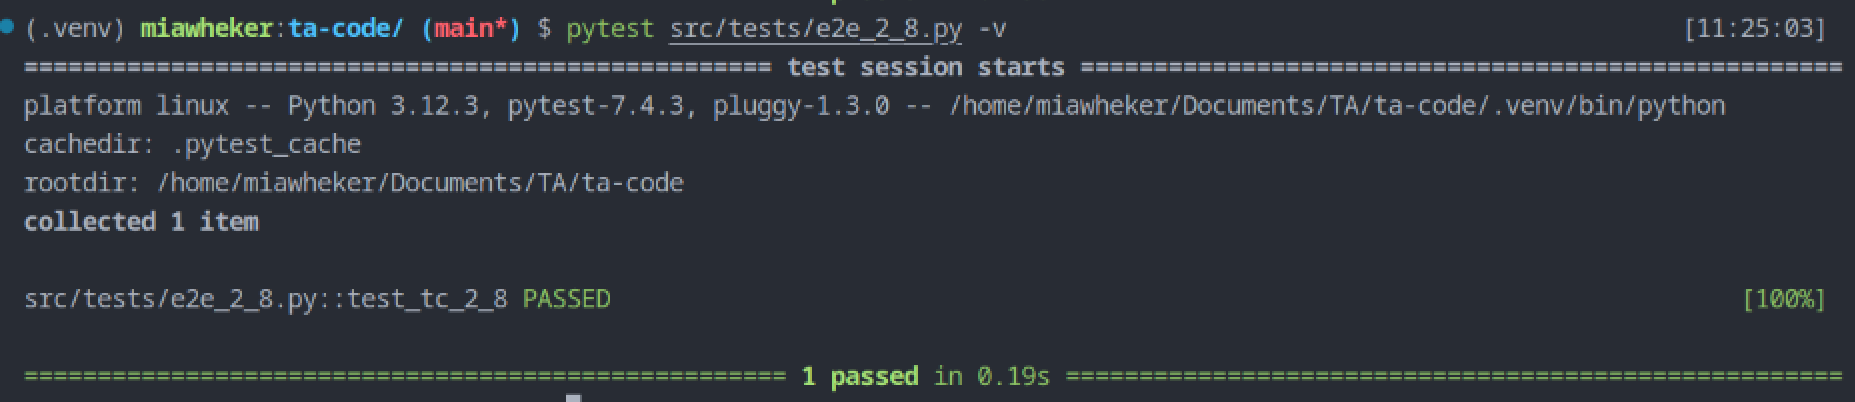
\includegraphics[width=\textwidth]{chapters/res/appendix-4/2.8.png}
  \caption{Hasil Pengujian Kasus Uji T2.8}
  \label{fig:unit.test.t2.8}
\end{figure}

\section{Kasus Uji T2.9}

Kasus uji ini menguji terkait dengan \emph{replay attack} pada protokol TLS. Pada kasus ini, protokol harus tetap dapat bekerja setelah mendapatkan \emph{replay attack}. Algoritme \ref{alg:unit.test.t2.9} menjelaskan terkait implementasi kasus uji ini. Hasil dari pengujian ini ditunjukan oleh gambar \ref{fig:unit.test.t2.9}. Pada gambar tersebut, terlihat bahwa pengujian berhasil.


\begin{algorithm}
  \caption{Algoritme Pengujian Kasus Uji T2.9}
  \label{alg:unit.test.t2.9}
  \begin{algorithmic}
    \State $cert, prk \gets generatePairCertificate()$
    \State $socket_1 \gets \text{UnixSocket}()$
    \State $socket_2 \gets \text{UnixSocket}()$
    \State $tls_{alice} \gets \text{TLSApplication}(socket_1, \text{'client'}, cert)$ 
    \State $tls_{bob} \gets \text{TLSApplication}(socket_2, \text{'server'}, cert, prk)$
    \State $mitm \gets \text{MITMProxy}(socket_1, socket_2)$
    \State
    \State $tls_{bob}.\text{listen}()$ \Comment {Bob melakukan listen pada socket} 
    \State $tls_{alice}.\text{connect}()$ \Comment {Alice dan Bob melakukan proses handshake} 
    \State
    \State $mitm.\text{forward}(2)$ \Comment {MITM meneruskan \emph{frame} ClientHello ke socket 2}
    \State $mitm.\text{forward}(1)$ \Comment {MITM meneruskan \emph{frame} ServerHello ke socket 1}
    \State $mitm.\text{forward}(1)$ \Comment {MITM meneruskan \emph{frame} Certificate ke socket 1}
    \State $mitm.\text{forward}(1)$ \Comment {MITM meneruskan \emph{frame} ServerKeyExchange ke socket 1}
    \State $mitm.\text{forward}(1)$ \Comment {MITM meneruskan \emph{frame} ServerHelloDone ke socket 1}
    \State $mitm.\text{forward}(2)$ \Comment {MITM meneruskan \emph{frame} ClientKeyExchange ke socket 2}
    \State $mitm.\text{forward}(2)$ \Comment {MITM meneruskan \emph{frame} ChangeCipherSpec ke socket 2}
    \State $mitm.\text{forward}(2)$ \Comment {MITM meneruskan \emph{frame} Finished (dari client)}
    \State $mitm.\text{forward}(1)$ \Comment {MITM meneruskan \emph{frame} ChangeCipherSpec ke socket 1}
    \State $mitm.\text{forward}(1)$ \Comment {MITM meneruskan \emph{frame} Finished (dari server)}
    \State
    \State $tls_{bob}.send(\text{'Hello, World!'})$
    \State $frame \gets mitm.\text{getFrame}()$
    \State $mitm.\text{send}(1, frame)$
    \State
    \State $tls_{alice}.\text{recv}(13)$ \Comment {Abaikan \emph{frame} ini}
    \State $mitm.\text{send}(1, frame)$ \Comment {Melakukan \emph{Replay Attack}}
    \State 
    \State $tls_{bob}.send(\text{'Hello, World!'})$
    \State $txt_{alice} \gets tls_{alice}.\text{recv}(13)$
    \State \textbf{assert} $txt_{alice} = \text{'Hello, World!'}$
  \end{algorithmic}
\end{algorithm}

\begin{figure}[ht]
  \centering
  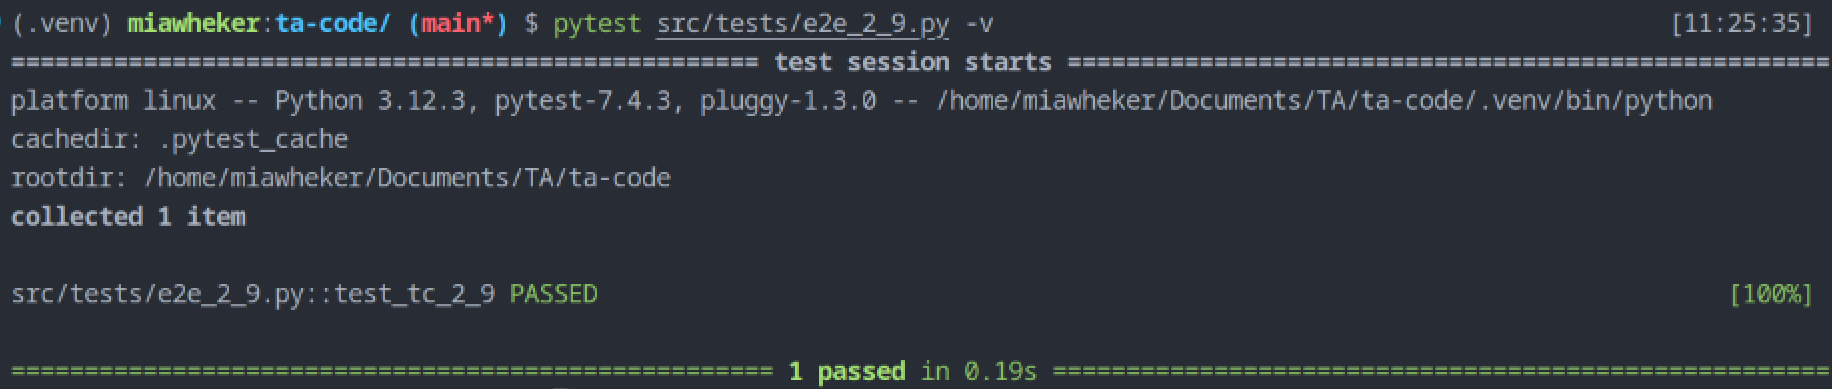
\includegraphics[width=\textwidth]{chapters/res/appendix-4/2.9.png}
  \caption{Hasil Pengujian Kasus Uji T2.9}
  \label{fig:unit.test.t2.9}
\end{figure}

\section{Kasus Uji T2.10}

Kasus uji ini menguji \emph{frame} dengan pesan yang sama memiliki hasil pesan yang berbeda. Proses ini dilakukan melalui aplikasi \emph{Wireshark}. Berikut merupakan skenario pengujian yang dilakukan:

\begin{enumerate}
  \item Melakukan koneksi ke \emph{echo server} dengan menggunakan protokol TLS.
  \item Melakukan \emph{capture} pada \emph{frame} yang dikirimkan.
  \item Mengirimkan pesan \texttt{Hello, World!} ke \emph{echo server} sebanyak dua kali.
\end{enumerate}

Hasil dari pengujian ini menunjukkan bahwa \emph{frame} yang dikirimkan memiliki nilai MAC dan pesan yang berbeda. Hal ini ditunjukan pada gambar \ref{fig:unit.test.t2.10}. Hal ini membuktikan bahwa pengujian berhasil.

\begin{figure}[ht]
  \centering
  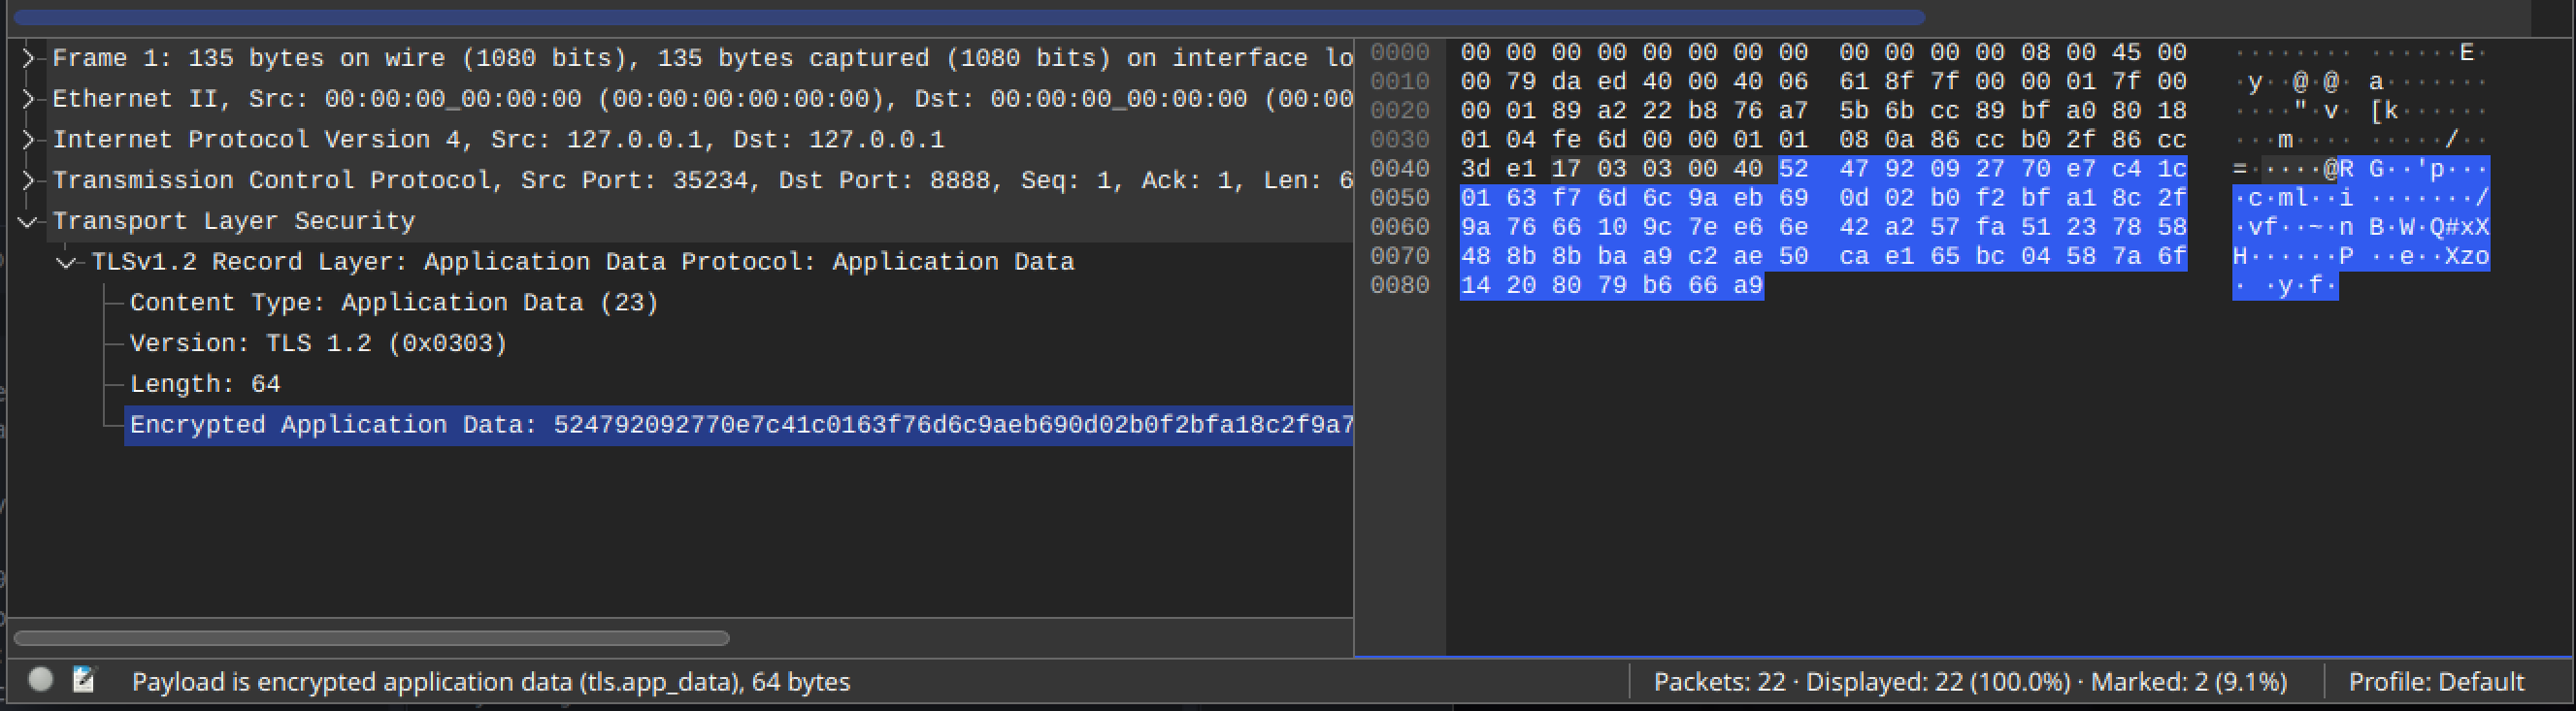
\includegraphics[width=\textwidth]{chapters/res/appendix-4/2.10.1.png}
  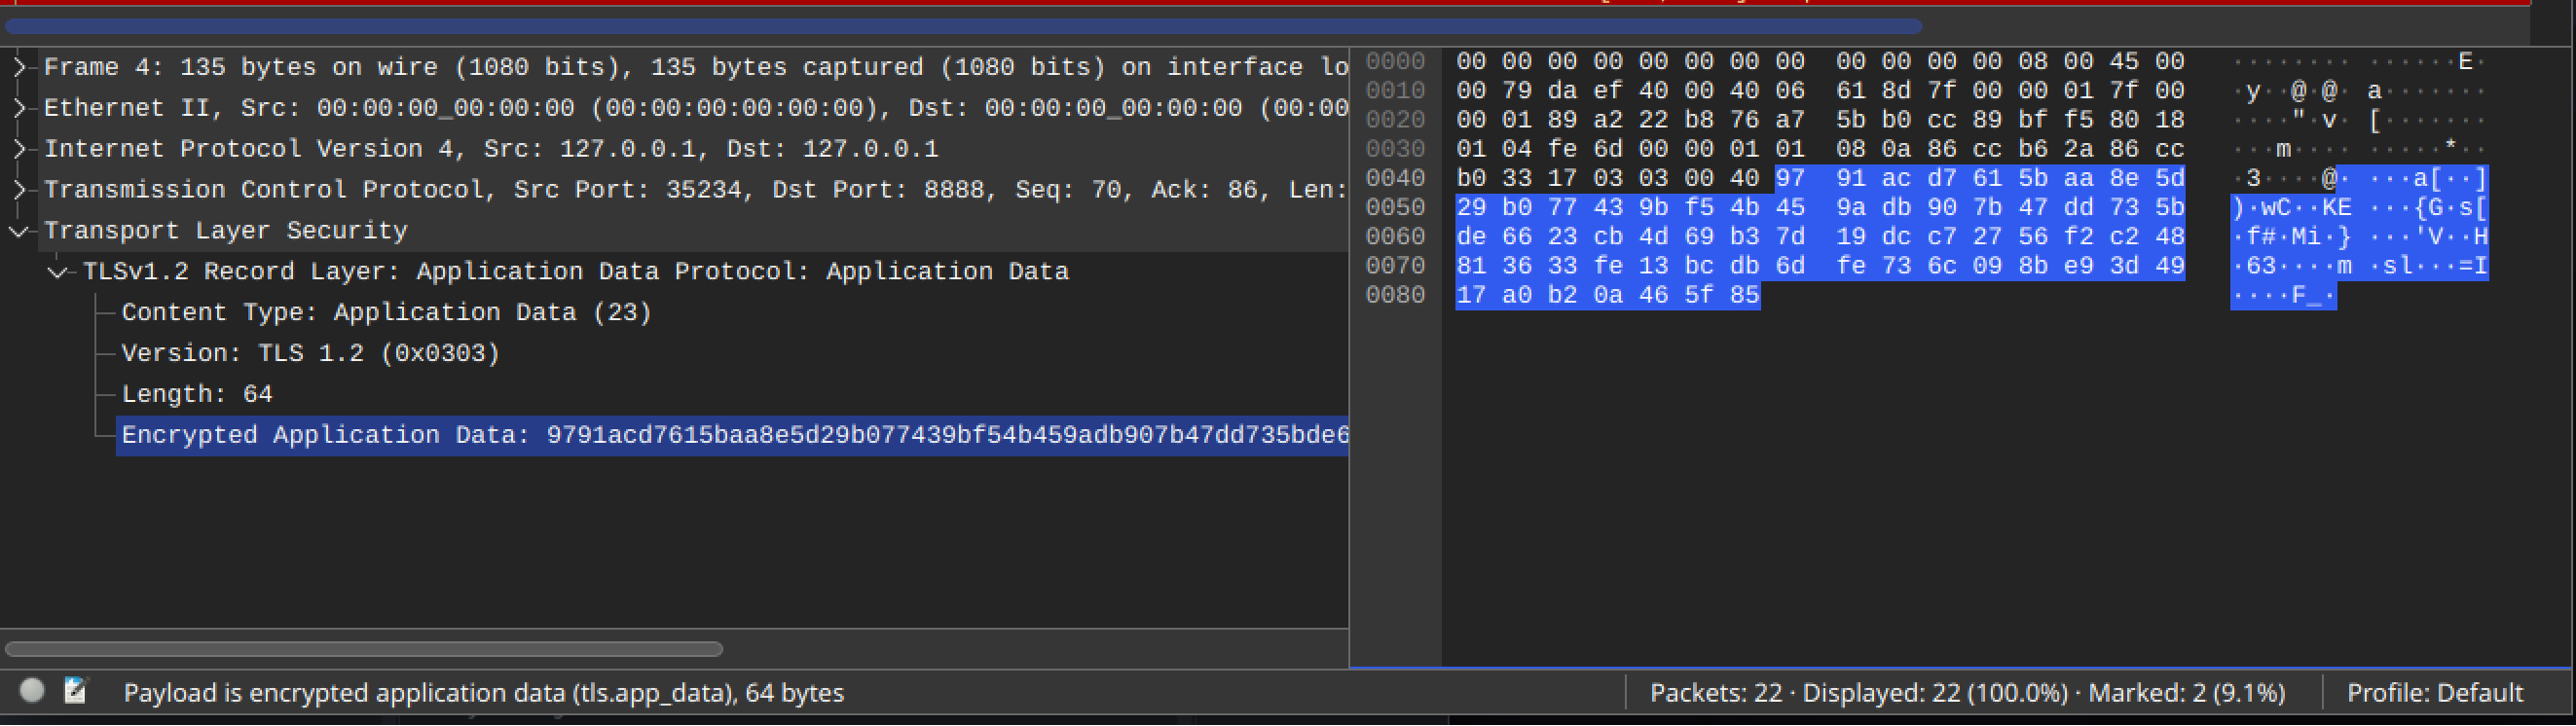
\includegraphics[width=\textwidth]{chapters/res/appendix-4/2.10.2.png}
  \caption{Hasil Pengujian Kasus Uji T2.10}
  \label{fig:unit.test.t2.10}
\end{figure}

\section{Kasus Uji T2.11}

Kasus uji ini menguji proses \emph{handshake} apabila dilakukan proses \emph{tampering} pada \emph{frame} \emph{ClientHello}. Algoritme \ref{alg:unit.test.t2.11} menjelaskan terkait implementasi kasus uji ini. Hasil dari pengujian ini ditunjukan oleh gambar \ref{fig:unit.test.t2.11}. Pada gambar tersebut, terlihat bahwa pengujian berhasil.

\begin{algorithm}
  \caption{Algoritme Pengujian Kasus Uji T2.11}
  \label{alg:unit.test.t2.11}
  \begin{algorithmic}
    \State $cert, prk \gets generatePairCertificate()$
    \State $socket_1 \gets \text{UnixSocket}()$
    \State $socket_2 \gets \text{UnixSocket}()$
    \State $tls_{alice} \gets \text{TLSApplication}(socket_1, \text{'client'}, cert)$ 
    \State $tls_{bob} \gets \text{TLSApplication}(socket_2, \text{'server'}, cert, prk)$
    \State $mitm \gets \text{MITMProxy}(socket_1, socket_2)$
    \State
    \State $tls_{bob}.\text{listen}()$ \Comment {Bob melakukan listen pada socket} 
    \State $tls_{alice}.\text{connect}()$ \Comment {Alice dan Bob melakukan proses handshake} 
    \State
    \State $hello \gets mitm.\text{getFrame}()$ \Comment {MITM mengambil \emph{frame} ClientHello}
    \State $hello.random.random_bytes \gets generateRandomBytes(28)$
    \State $mitm.\text{send}(2, hello)$
    \State
    \State $mitm.\text{forward}(1)$ \Comment {MITM meneruskan \emph{frame} ServerHello ke socket 1}
    \State $mitm.\text{forward}(1)$ \Comment {MITM meneruskan \emph{frame} Certificate ke socket 1}
    \State $mitm.\text{forward}(1)$ \Comment {MITM meneruskan \emph{frame} ServerKeyExchange ke socket 1}
    \State $mitm.\text{forward}(1)$ \Comment {MITM meneruskan \emph{frame} ServerHelloDone}
    \State $mitm.\text{forward}(2)$ \Comment {MITM meneruskan \emph{frame} ClientKeyExchange}
    \State $mitm.\text{forward}(2)$ \Comment {MITM meneruskan \emph{frame} Finished (dari client)}
    \State
    \State $alert \gets mitm.\text{getFrame}()$
    \State $mitm.\text{send}(1, alert)$
    \State
    \State \textbf{assert} $\lnot tls_{alice}.\text{handshakeSuccess} \land \lnot tls_{bob}.\text{handshakeSuccess}$
    \State \textbf{assert} $alert.\text{type} = \text{ContentType.alert}$
    \State \textbf{assert} $alert.\text{level} = \text{AlertLevel.fatal}$
    \State \textbf{assert} $alert.\text{description} = \text{AlertDescription.handshake\_failure}$
  \end{algorithmic}
\end{algorithm}

\begin{figure}[ht]
  \centering
  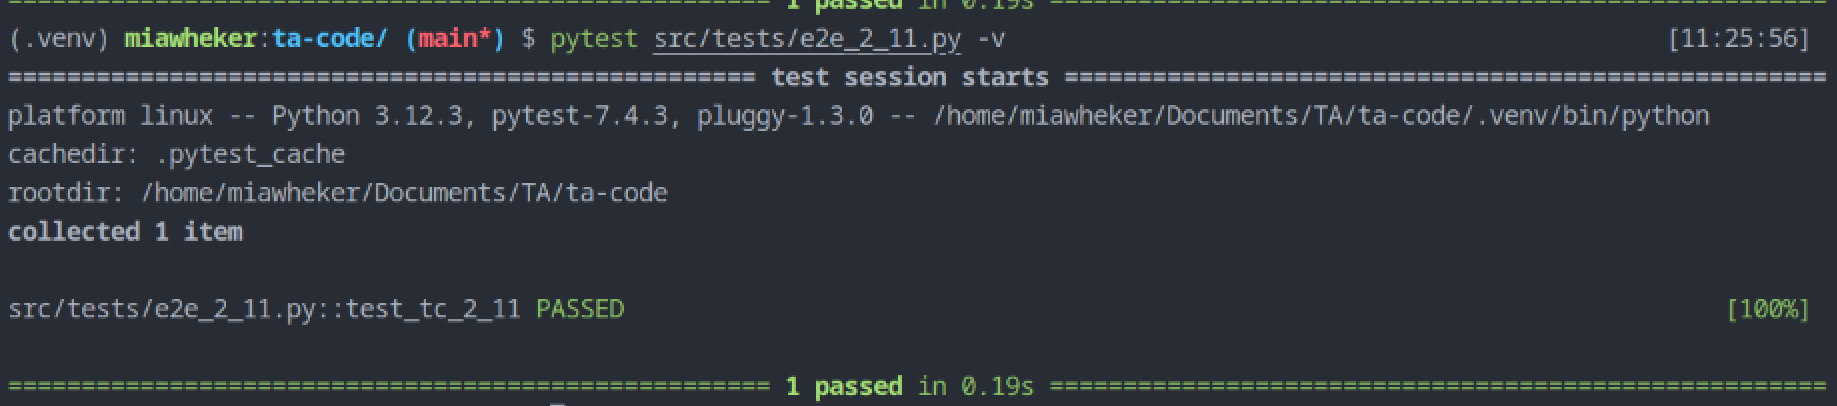
\includegraphics[width=\textwidth]{chapters/res/appendix-4/2.11.png}
  \caption{Hasil Pengujian Kasus Uji T2.11}
  \label{fig:unit.test.t2.11}
\end{figure}

\section{Kasus Uji T2.12}

Kasus uji ini menguji proses \emph{handshake} apabila dilakukan proses \emph{tampering} pada \emph{frame} \emph{ServerHello}. Algoritme \ref{alg:unit.test.t2.12} menjelaskan terkait implementasi kasus uji ini. Hasil dari pengujian ini ditunjukan oleh gambar \ref{fig:unit.test.t2.12}. Pada gambar tersebut, terlihat bahwa pengujian berhasil.


\begin{algorithm}
  \caption{Algoritme Pengujian Kasus Uji T2.12}
  \label{alg:unit.test.t2.12}
  \begin{algorithmic}
    \State $cert, prk \gets generatePairCertificate()$
    \State $socket_1 \gets \text{UnixSocket}()$
    \State $socket_2 \gets \text{UnixSocket}()$
    \State $tls_{alice} \gets \text{TLSApplication}(socket_1, \text{'client'}, cert)$ 
    \State $tls_{bob} \gets \text{TLSApplication}(socket_2, \text{'server'}, cert, prk)$
    \State $mitm \gets \text{MITMProxy}(socket_1, socket_2)$
    \State
    \State $mitm.\text{forward}(2)$ \Comment {MITM meneruskan \emph{frame} ClientHello ke socket 1}
    \State $tls_{bob}.\text{listen}()$ \Comment {Bob melakukan listen pada socket} 
    \State $tls_{alice}.\text{connect}()$ \Comment {Alice dan Bob melakukan proses handshake} 
    \State
    \State $hello \gets mitm.\text{getFrame}()$ \Comment {MITM mengambil \emph{frame} ServerHello}
    \State $hello.random.random_bytes \gets generateRandomBytes(28)$
    \State $mitm.\text{send}(1, hello)$
    \State $mitm.\text{forward}(1)$ \Comment {MITM meneruskan \emph{frame} Certificate ke socket 1}
    \State $mitm.\text{forward}(1)$ \Comment {MITM meneruskan \emph{frame} ServerKeyExchange ke socket 1}
    \State $mitm.\text{forward}(1)$ \Comment {MITM meneruskan \emph{frame} ServerHelloDone}
    \State $mitm.\text{forward}(2)$ \Comment {MITM meneruskan \emph{frame} ClientKeyExchange}
    \State $mitm.\text{forward}(2)$ \Comment {MITM meneruskan \emph{frame} Finished (dari client)}
    \State
    \State $alert \gets mitm.\text{getFrame}()$
    \State $mitm.\text{send}(1, alert)$
    \State
    \State \textbf{assert} $\lnot tls_{alice}.\text{handshakeSuccess} \land \lnot tls_{bob}.\text{handshakeSuccess}$
    \State \textbf{assert} $alert.\text{type} = \text{ContentType.alert}$
    \State \textbf{assert} $alert.\text{level} = \text{AlertLevel.fatal}$
    \State \textbf{assert} $alert.\text{description} = \text{AlertDescription.handshake\_failure}$
  \end{algorithmic}
\end{algorithm}

\begin{figure}[ht]
  \centering
  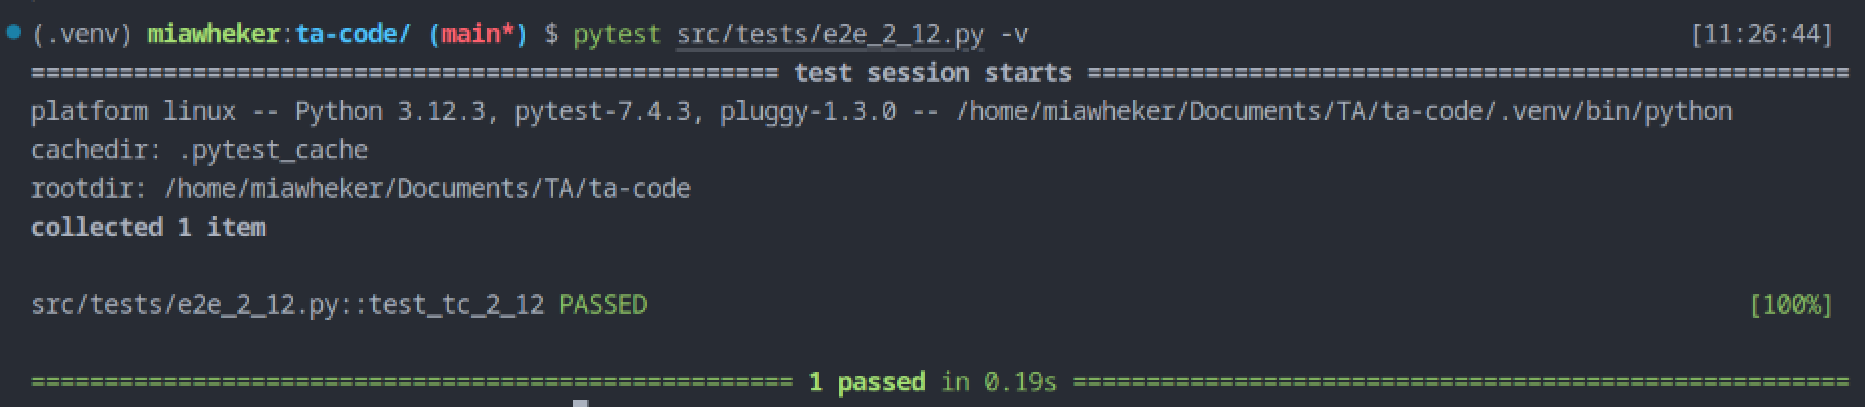
\includegraphics[width=\textwidth]{chapters/res/appendix-4/2.12.png}
  \caption{Hasil Pengujian Kasus Uji T2.12}
  \label{fig:unit.test.t2.12}
\end{figure}

\section{Kasus Uji T2.13}

Kasus uji ini menguji proses \emph{handshake} apabila \emph{certificate} yang dilakukan \emph{pinning} pada \emph{client} tidak sesuai dengan \emph{certificate} yang diterima dari \emph{server}. Algoritme \ref{alg:unit.test.t2.13} menjelaskan terkait implementasi kasus uji ini. Hasil dari pengujian ini ditunjukan oleh gambar \ref{fig:unit.test.t2.13}. Pada gambar tersebut, terlihat bahwa pengujian berhasil.

\begin{figure}[ht]
  \centering
  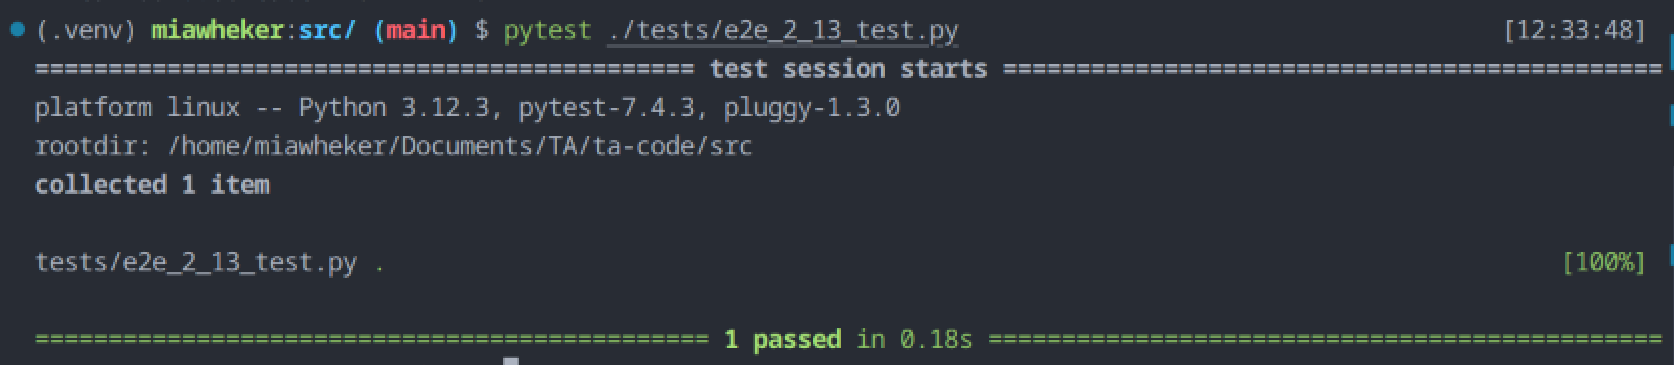
\includegraphics[width=\textwidth]{chapters/res/appendix-4/2.13.png}
  \caption{Hasil Pengujian Kasus Uji T2.13}
  \label{fig:unit.test.t2.13}
\end{figure}


\begin{algorithm}
  \caption{Algoritme Pengujian Kasus Uji T2.13}
  \label{alg:unit.test.t2.13}
  \begin{algorithmic}
    \State $cert_1, prk_1 \gets generatePairCertificate()$
    \State $cert_2, prk_2 \gets generatePairCertificate()$
    \State $socket \gets \text{UnixSocket}()$
    \State $tls_{alice} \gets \text{TLSApplication}(socket, \text{'client'}, cert_1)$ 
    \State $tls_{bob} \gets \text{TLSApplication}(socket, \text{'server'}, cert_2, prk_2)$
    \State
    \State $tls_{bob}.\text{listen}()$ \Comment {Bob melakukan listen pada socket} 
    \State $tls_{alice}.\text{connect}()$ \Comment {Alice dan Bob melakukan proses handshake} 
    \State
    \State
    \State \textbf{assert} $\lnot tls_{alice}.\text{handshakeSuccess} \land \lnot tls_{bob}.\text{handshakeSuccess}$
  \end{algorithmic}
\end{algorithm}
